\section{Dense Intelligence}
\label{sec:dense}

\begin{designbox}
Keep research intelligence \emph{dense} in time: hold decision, execution, and
verification coupled and continuous over persisted state, so that a long-horizon
program behaves as one sustained line of reasoning rather than a sequence of
disconnected bursts.
\end{designbox}

\subsection{Definition}

By \emph{dense intelligence} we mean sustained, coupled research work: at every
point in a long run the system is making decisions, carrying them into real
execution, and verifying the outcome against evidence --- and the thread that
connects these is never broken by the end of a model call. Sparse intelligence is
the default failure mode of a capable model left to run long: it is brilliant in
bursts and empty in between, because each burst ends and its working state is
discarded. Density is not about being busy; it is about the fraction of elapsed
research time in which genuine decisions are being made, executed, and checked,
rather than lost to context recovery, idle polling, or unverifiable self-report.
Figure~\ref{fig:dense} contrasts episodic research, where useful work is separated
by context-recovery gaps, with the continuous role loop that runs over persisted
project state.

\begin{figure}[H]
\centering
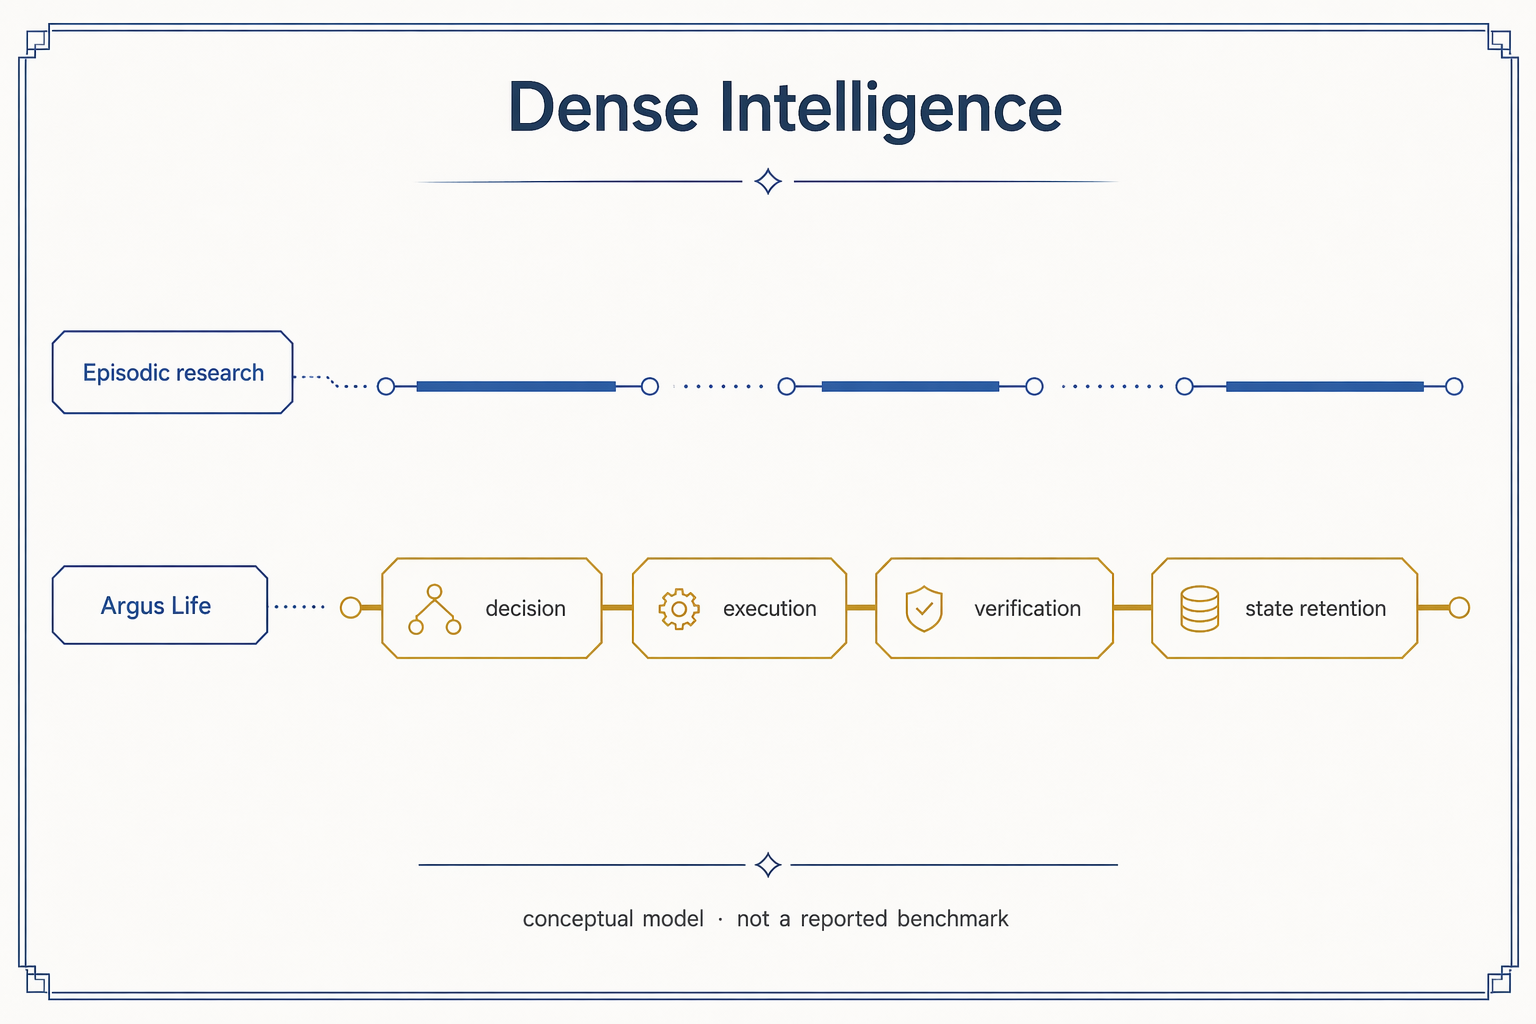
\includegraphics[width=0.82\textwidth]{figures/dense_intelligence.png}
\caption{Dense intelligence as continuity of coupled work. Episodic research
recovers decision and verification repeatedly across context gaps; Argus keeps
decision, execution, verification, and state retention coupled over a persisted
project. The schematic is a conceptual model, not a reported benchmark.}
\label{fig:dense}
\end{figure}

\subsection{Continuity is not token volume}

The tempting shortcut is to equate continuity with a larger context window: keep
more tokens live and the run will stay coherent. It will not. A longer window
lengthens a single episode but does nothing to couple decision to execution to
verification, and it still terminates --- at which point the accumulated working
state is compacted or dropped and the next episode restarts cold. Token volume
measures how much text a model can attend to at once; density measures how much of
a research horizon is spent on verified, decision-bearing work. A run can consume
enormous context and remain sparse --- re-reading the same files, re-deriving the
same dead ends --- because none of that volume is gated by an independent check or
retained as reusable capability. Continuity that matters is structural: it comes
from persisting state outside the model and cycling roles over it, not from
holding more tokens inside the model.

\subsection{A conceptual density model}

To make the idea precise enough to reason about --- and no more --- we summarize
it as a time-averaged density over a research horizon $T$:

\begin{equation}
\rho_{\mathrm{DI}}(T)
= \frac{1}{T}\int_0^T
\lambda(t)\,\eta_d(t)\,\eta_x(t)\,\eta_v(t)\,dt .
\end{equation}

The integrand multiplies a rate of research activity by three efficiencies, so
that time spent busy but undirected, or active but unverified, contributes little.

\begin{table}[H]
\small
\renewcommand{\arraystretch}{1.3}
\begin{tabularx}{\linewidth}{@{}c >{\raggedright\arraybackslash}X@{}}
\toprule
\textbf{Symbol} & \textbf{Meaning} \\
\midrule
$T$ & The research horizon over which density is averaged --- hours to days, not a
single call. \\
\addlinespace
$\lambda(t)$ & Instantaneous rate of research activity: how much work the system is
attempting at time $t$. \\
\addlinespace
$\eta_d(t)$ & Decision efficiency: the fraction of that activity that is a genuine
decision advancing the frontier rather than repetition. \\
\addlinespace
$\eta_x(t)$ & Execution efficiency: the fraction of decisions carried into real
execution on real tools, data, and hardware. \\
\addlinespace
$\eta_v(t)$ & Verification efficiency: the fraction of executed work that is
independently checked against evidence. \\
\bottomrule
\end{tabularx}
\caption{The five symbols of the conceptual density model.}
\label{tab:density}
\end{table}

Read this way, the episodic failure mode is exactly a collapse of one or more
efficiencies to near zero for long stretches: high $\lambda$ but low $\eta_d$
(busy, not deciding), or non-trivial $\eta_d$ and $\eta_x$ but low $\eta_v$
(acting, not verifying). The design of Argus is an attempt to hold all three
efficiencies away from zero across the whole horizon by construction --- persistent
roles for decision and verification, real execution for $\eta_x$, and an evidence
gate for $\eta_v$.

\subsection{What is and is not measured}

The model above is a lens, not an instrument. $\rho_{\mathrm{DI}}$ is an
explanatory construct, not a reported benchmark metric. It does not, in itself,
establish that Argus is universally superior to human researchers or other
systems. No number in this report is a measurement of $\rho_{\mathrm{DI}}$: the
integrand's efficiencies are not instrumented as a live scalar, and we make no
attempt to publish one. What \emph{is} measured is reported elsewhere under
explicit protocols --- the six public arena results and the 41-paper portfolio of
Section~\ref{sec:results} and Section~\ref{sec:portfolio}, each a scoped claim
under its stated evidence tier. Dense intelligence is the design goal those
results are evidence \emph{for}; it is not itself a score, and it is not a claim of
general superiority.
